\documentclass[12pt]{article}
\usepackage[utf8]{inputenc}
\usepackage[russian]{babel}
\usepackage[OT1]{fontenc}
\usepackage{amsfonts, amsmath, amsthm, amssymb}
\usepackage[left=1cm,right=1cm,top=1cm,bottom=2cm]{geometry}
\usepackage{paralist}
\usepackage{graphicx}

\newcounter{problem}
\newcommand{\z}{\par  \smallskip \noindent \refstepcounter{problem}%
\textbf{Problem №\arabic{problem}.} }

\def\sol{\par \bigskip \noindent \textbf{Solution. }}
\def\solI{\noindent \textbf{First solution. }}
\def\solII{\par \noindent \textbf{Second solution. }}
\def\solIII{\par \noindent \textbf{Third solution. }}
\def\lemmaI{\noindent \textbf{Lemma. }}
\def\lemma#1{\noindent \textbf{Lemma {#1}. }}
\def\proof{\par \noindent \textbf{Proof. }}

\DeclareRobustCommand{\divby}{%
  \mathrel{\text{\vbox{\baselineskip.65ex\lineskiplimit0pt\hbox{.}\hbox{.}\hbox{.}}}}%
}

\begin{document}

\centerline{\sc \textbf{XIX Silk Road Mathematical Competition}}

\centerline{\sc \textbf{March 2020}}

\bigskip
\hrule
\bigskip

\textsl{\textbf{Attention!} 
We ask you not to \textbf{disclose} these problems and not to discuss them publicly (especially through Internet) before May 25, 2020.}

\bigskip

\centerline{\sc \textbf{Solutions and marking schemes}}

\bigskip

\z An infinite strictly increasing sequence of positive integers $\{a_n\}_{n \geq 1}$ is given. It is also given that $a_n \leq n + 2020$ and $n^3 a_n - 1$ is divisible by $a_{n+1}$ for any positive integer $n$. Prove that $a_n = n$ for any positive integer $n$. \textit{(Kanat Satylkhanov)}

\bigskip

\solI By induction on $n$ it is easy to show that $a_n \geq n$ for any $n$. Suppose that there exists a positive integer $k$ such that $a_k > k$. Let's choose such positive integer $m$ that $m \divby 2021!$ and $m > k$. Then for any $i = 2, 3, \ldots, 2021$, GCD$(m, m+i) > 1$. It follows from the problem statement that GCD$(m, a_{m+1})=1$. Since $\{a_n\}$ is strictly increasing and $a_k > k$, then $a_{m+1} > m+1$. Therefore, $m + 2 \leq a_{m+1} \leq m + 2021$, but then GCD$(m, a_{m+1}) > 1$ --- a contradiction.

\bigskip

\textbf{Marking scheme.}
\begin{compactitem}
\item Consideration of a positive integer that is divisible by each of the numbers $2, 3, \ldots, 2021$ --- 2 points
\item Proof that for any positive integer $k$ there exists such positive integer $m > k$ that $a_m = m$ --- 6 points
\item These items are not additive
\end{compactitem}

\bigskip

\solII Let $b_n = a_n - n$ for each $n$. By induction on $n$ it is easy to show that $b_n \geq 0$ for any $n$. If $b_k > b_{k+1}$ for some $k$, then 
\[a_k - k > a_{k+1} - k - 1 \implies a_k + 1 > a_{k+1} \implies a_k \geq a_{k+1}\]
--- a contradiction. Thus, the sequence $\{b_n\}$ is non-decreasing. On the other hand, it has an upper bound: $b_n = a_n - n \leq 2020$. Hence, there exists such non-negative integer $k$ and a positive integer $t$ that $b_n = k$ for each $n \geq t$. So, for any $n \geq t$
\[a_{n+1} \ | \ n^3 a_n - 1 \implies n + k + 1 \ | \ n^3 (n + k) - 1 \implies\]
\[\implies n + k + 1 \ | \ n^3 (n + k) - 1 - (n + k + 1)(n^3 - n^2 + n(k+1) - (k+1)^2) = (k + 1)^3 - 1 \implies\]
\[\implies n + k + 1 \ | \ (k + 1)^3 - 1.\]
But this is only possible when $k = 0$. Therefore, $b_n = 0$ for each sufficiently large $n$, and thus for all $n$, i. e. $a_n = n$ for all $n$.

\bigskip

\textbf{Marking scheme.}
\begin{compactitem}
\item (1) Proof that $b_k \leq b_{k+1}$ for any $k$ --- 1 point
\item (2) Proof that $\{b_n\}$ is constant after some point --- 3 points
\item (3) Proof that $b_n = 0$ after some point --- 3 points
\item Items (1) and (2) are not additive
\end{compactitem}

\bigskip

\z Triangle $ABC$ is inscribed into circle $\omega$. On sides $AB$, $BC$, $CA$ there are points $K, L, M$, respectively, such that $CM \cdot CL = AM \cdot BL$. Ray $LK$ intersects line $AC$ at point $P$. The common chord of $\omega$ and the circumscribed circle of $KMP$ intersects segment $AM$ at point $S$. Prove that $SK \parallel BC$. \textit{(Medeubek Kungozhin)}

\bigskip

\solI 

\bigskip

{
\centerline {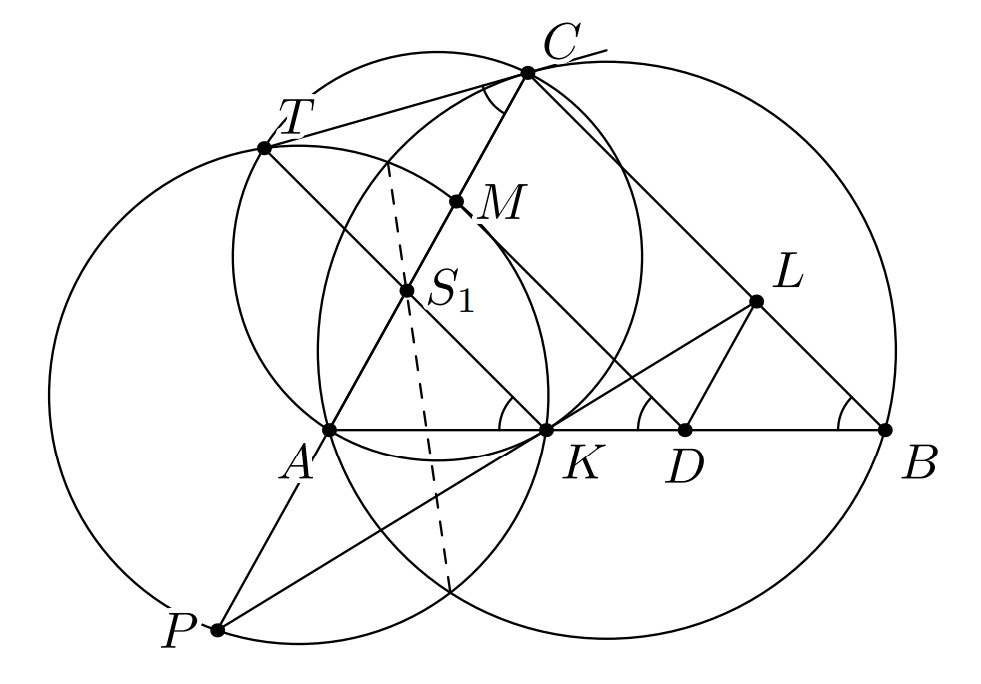
\includegraphics[scale=0.5]{img_1.jpg}}
}

\bigskip

\noindent Suppose that $AC \leq BC$. Let $D$ be a point on the side $AB$ such that $DM \parallel BC$. Then 
\[\frac{DB}{DA} = \frac{CM}{AM} = \frac{BL}{CL},\]
i. e. $DL \parallel AC$. On the tangent line to $\omega$ at point $C$ let's choose a point $T$, such that $KT \parallel BC$. Then $\angle TKA = \angle CBA = \angle TCA$. Therefore, $AKCT$ is cyclic. Let segments $KT$ and $AC$ intersect at point $S_1$. Then
\[\frac{S_1P}{S_1C} = \frac{KP}{KL} = \frac{KA}{KD} = \frac{S_1A}{S_1M} \implies S_1P \cdot S_1M = S_1C \cdot S_1A = S_1K \cdot S_1T.\]
Thus, $TMKP$ is inscribed into the circumcircle of triangle $KMP$. It is known that the common chords of three pairs of circles, centers of which are not collinear, are concurrent. It means that the common chord of $\omega$ and the circumcircle of $KMP$ passes through point $S_1$. Therefore, point $S_1$ coincides with $S$, and $S_1K \parallel BC$ follows from the definition of $T$. 

\bigskip

\textbf{Marking scheme.}
\begin{compactitem}
\item Proof that $DL \parallel AC$ --- 0 points
\item Consideration of point $T$ --- 1 point
\item Proof that $P, K, M, T$ lie on the same circle --- 4 points
\end{compactitem}

\bigskip

\solII Let's introduce some notation:
\[b = AC, \ m = AM, \ s = AS, \ p = AP.\]
Since $S$ lies on the radical axis of the circumcircles of $ABC$ and $PKM$, then
\[SM \cdot SP = SA \cdot SC \implies (m - s)(s + p) = s(b - s) \implies s = \frac{pm}{b + p - m}.\]
So,
\[\frac{AS}{SC} = \frac{s}{b - s} = \frac{pm}{(b - m)(b + p)}.\]
According to Menelaus' theorem for triangle $ABC$ and transversal line $PKL$:
\[\frac{AK}{KB} \cdot \frac{BL}{LC} \cdot \frac{CP}{PA} = 1 \implies \frac{AK}{KB} = \frac{CL}{LB} \cdot \frac{AP}{PC} = \frac{AM}{MC} \cdot \frac{AP}{PC} = \frac{m}{b - m} \cdot \frac{p}{b + p} = \frac{AS}{SC} \implies SK \parallel BC,\]
Q. E. D.

\bigskip

\textbf{Marking scheme.}
\begin{compactitem}
\item Unfinished computational solution --- 0 points
\end{compactitem}

\bigskip

\z Polynomial $Q(x) = k_n x^n + k_{n-1} x^{n-1} + \ldots + k_1 x + k_0$ with real coefficients is called \textit{mighty} if $|k_0| = |k_1| + |k_2| + \ldots + |k_{n-1}| + |k_n|$, and \textit{non-increasing} if $k_0 \geq k_1 \geq \ldots \geq k_{n-1} \geq k_n$. 

Let $P(x) = a_d x^d + a_{d-1} x^{d-1} + \ldots + a_1 x + a_0$ be a polynomial with real non-zero coefficients, such that $a_d > 0$ and $P(x)(x-1)^t(x+1)^s$ is \textit{mighty} for some non-negative integers $s$ and $t$ ($s + t > 0$). Prove that at least one of the polynomials $P(x)$ and $(-1)^d P(-x)$ is \textit{non-increasing}. \textit{(Navid Safaei, Iran)}

\bigskip

\sol Note that if for some real numbers $x_1, x_2, \ldots, x_m$ the following equality holds:
\[|x_1| + |x_2| + \ldots + |x_m| = |x_1 + x_2 + \ldots + x_m|,\]
then they are of the same sign.

Let
\[Q(x) = P(x) (x-1)^t (x+1)^s = b_n x^n + b_{n-1} x^{n-1} + \ldots + b_0,\]
where $b_n = a_d > 0$. From the problem statement it follows that 
\[|b_0| = |b_1| + |b_2| + \ldots + |b_n|.\]

\textbf{Lemma:} If $t \geq 1$, then $b_1, b_2, \ldots, b_n \geq 0$.

\textbf{Proof:} 
\[Q(1) = 0 \implies b_0 + b_1 + \ldots + b_n = 0 \implies\] 
\[\implies |b_1 + b_2 + \ldots + b_n| = |b_0| = |b_1| + |b_2| + \ldots + |b_n|,\]
hence, $b_1, b_2, \ldots, b_n$ are of the same sign. Since $b_n > 0$, then $b_1, b_2, \ldots, b_{n-1} \geq 0$. We proved the lemma.

Assume that $t \geq 2$. According to the lemma,
\[b_1, b_2, \ldots, b_{n-1} \geq 0 \implies b_1 + 2b_2 + \ldots + nb_n > 0.\] 
On the other hand, let $R(x) = \dfrac{Q(x)}{(x - 1)^2}$. Then
\[Q'(x) = 2(x - 1) R(x) + (x - 1)^2 R'(x) \implies Q'(1) = 0 \implies b_1 + 2b_2 + \ldots + nb_n = 0\]
--- a contradiction. Thus, $t \leq 1$.

Similarly, we can show that $s \leq 1$. Let's consider three cases.

\textbf{I)} $t = 1, s = 1$. 
\[Q(x) = P(x) (x^2 - 1) \implies Q(1) = Q(-1) = 0 \implies \]
\[\implies b_0 + b_1 + \ldots + b_n = b_0 - b_1 + b_2 + \ldots + {(-1)^n} b_n = 0 \implies\]
\[\implies b_1 + b_3 + b_5 + \ldots = 0.\]
According to the lemma,
\[b_1, b_2, \ldots, b_n \geq 0 \implies b_1 = b_3 = b_5 = \ldots = 0,\]
--- a contradiction, since $b_1 = -a_1$ and by the problem statement $a_1 \neq 0$. 

\textbf{II)} $t = 1, s = 0$.
\[Q(x) = P(x)(x-1) = -a_0 + (a_0 - a_1 ) x + \ldots + (a_{d-1} - a_d) x^d + a_d x^{d+1}.\]
By the lemma,
\[a_0 - a_1 = b_1 \geq 0, \ldots, a_{d-1} - a_d = b_d \geq 0 \implies a_0 \geq a_1 \geq \ldots \geq a_d.\]
Therefore, $P(x)$ is non-increasing.

\textbf{III)} $t = 0, s = 1$.
\[Q(-1) = 0 \implies b_0 - b_1 + \ldots + (-1)^n b_n = 0 \implies\]
\[\implies |b_1 - b_2 + \ldots + (-1)^n b_n| = |b_0| = |b_1| + |-b_2| + \ldots + |(-1)^n b_n|.\]
Thus, $b_1, -b_2, \ldots, (-1)^n b_n$ are of the same sign, and since $b_n > 0$, then $(-1)^{n-i} b_i \geq 0$ for each $1 \leq i \leq n$. 
\[Q(x) = P(x)(x+1) = a_0 + (a_0 + a_1) x + \ldots + (a_{d-1} + a_d) x^d + a_d x^{d+1} \implies\]
\[\implies (-1)^{d+1-i} (a_{i-1} + a_i) \geq 0 \ (\text{for all } 1 \leq i \leq d) \implies\]
\[\implies a_d \leq -a_{d-1} \leq a_{d-2} \leq \ldots \leq (-1)^d a_0.\]
It follows that $(-1)^d P(-x) = a_d x^d - a_{d-1} x^{d-1} + \ldots + (-1)^d a_0$ is non-increasing.

\bigskip

\textbf{Marking scheme.}
\begin{compactitem}
\item (1) Proof of the \textbf{lemma} --- 2 points
\item (2) Proof that $t \leq 1$ and $s \leq 1$ --- 4 points
\item (3) Proof that $t \leq 1$ or $s \leq 1$ --- 3 points
\item (4) Consideration of the case $t = s = 1$ --- 1 point
\item (5) Consideration of the case $t = 1, s = 0$ --- 1 point
\item (6) Consideration of the case $t = 0, s = 1$ --- 1 point
\item Item (1) is not additive with any other one
\item Items (2) and (3) are not additive
\end{compactitem}

\bigskip

\z Prove that for any positive integer $m$ there exists a positive integer $n$, such that any $n$ different points on a plane can be partitioned into $m$ non-empty sets, \textit{convex hulls} of which would share a common point.

\textit{Convex hull} of a finite set $X$ of points on a plane is a set of points that lie inside or on the border of at least one convex polygon with vertices in $X$, including degenerate ones, i. e. a segment and a point are considered to be convex polygons. No three vertices of a convex polygon are collinear. A polygon contains its border. \textit{(Alikhan Zimanov)}

\bigskip

\solI Let's remind \textbf{Helly's theorem}: if in a finite set of convex sets of points on a plane each three intersect, then all of them intersect.

Let's prove that $n = 9m$ satisfies the problem statement. Let $X$ be an arbitrary set of $9m$ different points on a plane, and $Y$ --- the set of subsets of $X$ of size $6m + 1$. 

Suppose that there exist such $A, B, C \in Y$ that their intersection is empty. Let's enumerate all points in $X$ by numbers from 1 to $9m$. Let's write down on a sheet of paper the numbers of points in $A$, then the numbers of points in $B$, and after that the numbers of points in $C$. We wrote $|A| + |B| + |C| = 18m + 3$ numbers in total. Since these sets do not intersect, then we couldn't write any number more than twice. Thus, we wrote no more than $2 \cdot 9m = 18m$ numbers --- a contradiction. Therefore, any three elements of $Y$ intersect.

Since the convex hull of a set of points contains the set itself, then the convex hulls of any three elements of $Y$ intersect. According to Helly's theorem, the convex hulls of all elements of $Y$ share some common point $O$.

Let's prove the following \textbf{lemma}: if the convex hull of a finite set of points $Z$ contains some point $P$, then there exists such $W \subseteq Z$ that $|W| \leq 3$ and the convex hull of $W$ contains $P$. By definition of convex hull, there exists a convex polygon with the set of vertices $V \subseteq Z$ (possibly, degenerate) that contains $P$. If $|V| \leq 3$, then $V$ works as $W$. Otherwise, let's perform an arbitrary triangulation of the polygon with vertices in $V$. Point $P$ has to lie in at least one of the obtained triangles. The set of vertices of such triangle works as $W$.

Suppose we have a bag into which we can put non-empty subsets of $X$. Let's denote the following operation, which modifies $X$ and $Y$: take any $A \in Y$. Since the convex hull of $A$ contains $O$, then, according to the lemma, there exists such $B \subseteq A$ that $|B| \leq 3$ and the convex hull of $B$ contains $O$. Let's put $B$ into our bag (obviously, $B$ is non-empty), delete elements of $B$ from $X$, and delete sets from $Y$ that contain element of $B$. 

After one such operation the size of $X$ decreases by at most three, and $Y$ remains non-empty as long as $|X| \geq 6m + 1$. Therefore, we can perform the operation at least $m$ times. Let's perform it exactly $m$ times. Distribute the remaining elements of $X$ randomly among the sets in the bag. 

So, the sets in the bag constitute a partition of the initial set of points into $m$ non-empty sets and the convex hull of each of them contains point $O$, which is what we wanted.

\bigskip

\textbf{Marking scheme.}
\begin{compactitem}
\item Proof that the convex hulls of all subsets of size $\left[\dfrac{2n}{3}\right] + 1$ share a common point --- 3 points
\item Proof of the \textbf{lemma} --- 1 point
\item Usage of the \textbf{lemma} without proof --- minus 1 point
\item Correct partition without proof of correctness --- 2 points
\end{compactitem}

\bigskip

\solII Let's prove by induction on $m$ that any finite set of at least $4m^2$ different points on a plane can be partitioned into $m$ non-empty sets, convex hulls of which intersect. Obviously, the claim holds for $m = 1$. Assume that it holds for $m = k - 1$, where $k \geq 2$. Let's prove that it also holds for $m = k$. Let's consider an arbitrary finite set $X$ consisting of at least $4k^2$ different points on a plane. Let $Y$ be the subset of points of $X$ that lie on the border of the convex hull of $X$. If $|Y| < 4k$, then $|X \setminus Y| > 4k^2 - 4k > 4(k-1)^2$. By the induction hypothesis, $X \setminus Y$ can be partition into $k - 1$ non-empty sets, convex hulls of which intersect. If we add $Y$ to these $k - 1$ sets, then we would get $k$ sets, convex hulls of which intersect (since the convex hull of $Y$ contains all points from $X \setminus Y$).

If $|Y| \geq 4k$, then there are two cases. If all points from $Y$ lie on the same line, then all points from $X$ lie on the same line. Let's draw a coordinate axis along this line and denote the points from $X$ by $A_1, A_2, \ldots, A_{|X|}$ in the order of increasing coordinates. Since $4k^2 > 2k$, then the following partition works:
\[X = \{A_1, A_{|X|}\} \cup \{A_2, A_{|X|-1}\} \cup \ldots \cup \{A_{k-1}, A_{|X|-k+2}\} \cup \{A_k, A_{k+1}, \ldots, A_{|X|-k+1}\}\]

Otherwise points of $Y$ lie on the border of some non-degenerate convex polygon. Denote the points from $Y$ in clockwise order by 
\[A_1, A_2, \ldots, A_k, B_k, B_{k-1}, \ldots, B_1, C_1, C_2, \ldots, C_k, D_k, D_{k-1}, \ldots, D_1, E_1, E_2, \ldots, E_{|Y| - 4k}.\]
Let 
\[Z = \{A_k, B_k, C_k, D_k, E_1, \ldots, E_{|Y| - 4k}\} \cup (X \setminus Y).\]
Let's prove that the following partition works:
\[X = \left(\bigcup_{i=1}^{k-1} \{A_i, B_i, C_i, D_i\}\right) \cup Z.\]
It is enough to prove the \textbf{key assertion}: convex hulls of 
\[\{A_1, B_1, C_1, D_1\}, \{A_2, B_2, C_2, D_2\}, \ldots, \{A_k, B_k, C_k, D_k\}.\]
intersect. Denote the convex hull of a set of points $M$ by $f(M)$. Let
\[T \in A_1B_1 \cap A_kD_k,\]
\[H_i = f(\{A_1, A_2, \ldots, A_i, B_i, B_{i-1}, \ldots, B_1, C_1, C_2, \ldots, C_i, D_i, D_{i-1}, \ldots, D_1\})\]
and
\[V_i = f(\{A_i, A_{i+1}, \ldots, A_k, B_k, B_{k-1}, \ldots, B_i, C_i, C_{i+1}, \ldots, C_k, D_k, D_{k-1}, \ldots, D_i\}).\]
Then for each $1 \leq i \leq k$ holds
\[T \in A_1B_1 \subseteq H_i \ \text{and} \ T \in A_kD_k \subseteq V_i.\]
Therefore,
\[T \in \bigcap_{i=1}^{k} (H_i \cap V_i) = \bigcap_{i=1}^{k} f(\{A_i, B_i, C_i, D_i\}),\]
Q. E. D.

\bigskip

\textbf{Marking scheme.}
\begin{compactitem}
\item Reduction to the proof of the \textbf{key assertion} --- 4 points
\item Proof of the \textbf{key assertion} --- 3 points
\end{compactitem}

\bigskip

\end{document}
